\documentclass[a4paper,11pt,titlepage]{jsarticle}
\usepackage{amsmath,amssymb}
\usepackage{bm}
\usepackage[dvipdfmx]{graphicx}
\usepackage{here}
\usepackage{listings,jlisting}

%テキストの表示領域の調節
\setlength{\textwidth}{\paperwidth}
\addtolength{\textwidth}{-40truemm}
\setlength{\textheight}{\paperheight}
\addtolength{\textheight}{-45truemm}

%余白の調節
\setlength{\topmargin}{-10.4truemm}
\setlength{\evensidemargin}{-5.4truemm}
\setlength{\oddsidemargin}{-5.4truemm}
\setlength{\headheight}{17pt}
\setlength{\headsep}{10mm}
\addtolength{\headsep}{-17pt}
\setlength{\footskip}{5mm}

\title{5.ミドルウェアを用いた移動ロボットの知覚制御}
\author{1610004 青木 良太}
\date{提出日 2018年7月5日} % 省略可
\begin{document}
\maketitle

\section{実験の目的}
現代のロボットは複雑なシステム構成となっており, センサー, 信号処理, 認識, 行動決定, エンドエフェクタなどの様々なシステムが統合されている。そのため、
ロボットの開発では個々のシステムへの知識のみならず、それらを統合しシステムとして組み上げる能力が必要とされているが, それら全てを開発し, 統合することは非常に困難である.
そこで, ロボット開発に必要な様々な機能を備えた'ミドルウェア(ROS)'を用いることで, より容易にロボットシステム開発が可能になる.
本実験では移動ロボットの知覚制御を通して実際にミドルウェアを使用し, ロボットシステム開発の流れを学ぶことを目的とする。

\section{原理}
\subsection{ミドルウェア(ROS)}
ミドルウェア(ROS)とは, ロボットシステム開発を支援するライブラリとツールを提供するオープンソースソフトウェアのことである.
ROSの登場以前では, 様々なロボットが各開発環境において独自に開発されていたが, ROSの登場により, 汎用性の高いプログラムがより容易に
書くことが可能になった. また, 多くの開発者による研究がパッケージとしてROSに公開されており, パッケージを使うことで,
様々な機能の実装を簡単に行うことができるため, 少ない知識でも高度なロボットシステム開発が可能である.
現在では多数のロボット開発に使用されており, ソフトバンクロボティスクの「Pepper」なども、ROSに対応している.

\subsection{音声認識}
音声認識とは, 発声された音を文字列に変換する処理のことである. 音声認識をするためには音響モデルと認識辞書
が必要である. 音響モデルとは, 平均的発声データを基に作られた人間の発声の小さな単位(音素)の音響特徴が記述されている辞書のことである.
認識辞書には音声認識させることばが記述されている辞書である. 音声が入力されると音声を分析し, 音響特徴を算出した後に
認識辞書に記述されている言葉の中から, 言葉の音響特徴が入力音声の音響特徴に最も近い言葉を探して音声認識結果として出力します.

\subsection{画像認識}
画像認識とは, 画像や動画から特徴をつかみ, コンピュータに対象物を識別させるパターン認識技術の1つである.
コンピュータからすれば画像はピクセルの集合体に過ぎないため, ピクセルを塊(パターン)として認識させる必要がある.
また, 画像認識を行う前には画像処理を施さなけらばならない. 画像処理は, カメラによって取得された画像を処理するディジタル信号処理の技術であり,
ノイズ除去やエッジ検出、色の補正、2値化など多種多様な処理がある. 画像処理を施した後に, 画像中から物体を判別するために必要な特徴量を計算し,
その結果をパターン識別器で識別することで物体や人物を認識することが可能となる.

\section{実験装置}
\subsection{カメラセンサー}
Kinect(Microsoft製,図1)を用いて画像認識を行った. 以下の4つの機能を可能にした.
\begin{itemize}
  \item 人間骨格の認識:人間の骨格を認識と表示, 腕の位置(右手と左手がそれぞれ上, 前, 横のどこにあるか)の判別
  \item 顔の認識:人間の顔を検出し, 追跡
  \item 色の認識:赤色と青色を認識, 判別(図2)
  \item 物体の認識:あらかじめ登録しておいた物体を検出, 追跡(図3)
\end{itemize}

\begin{figure}[H]
  \begin{center}
    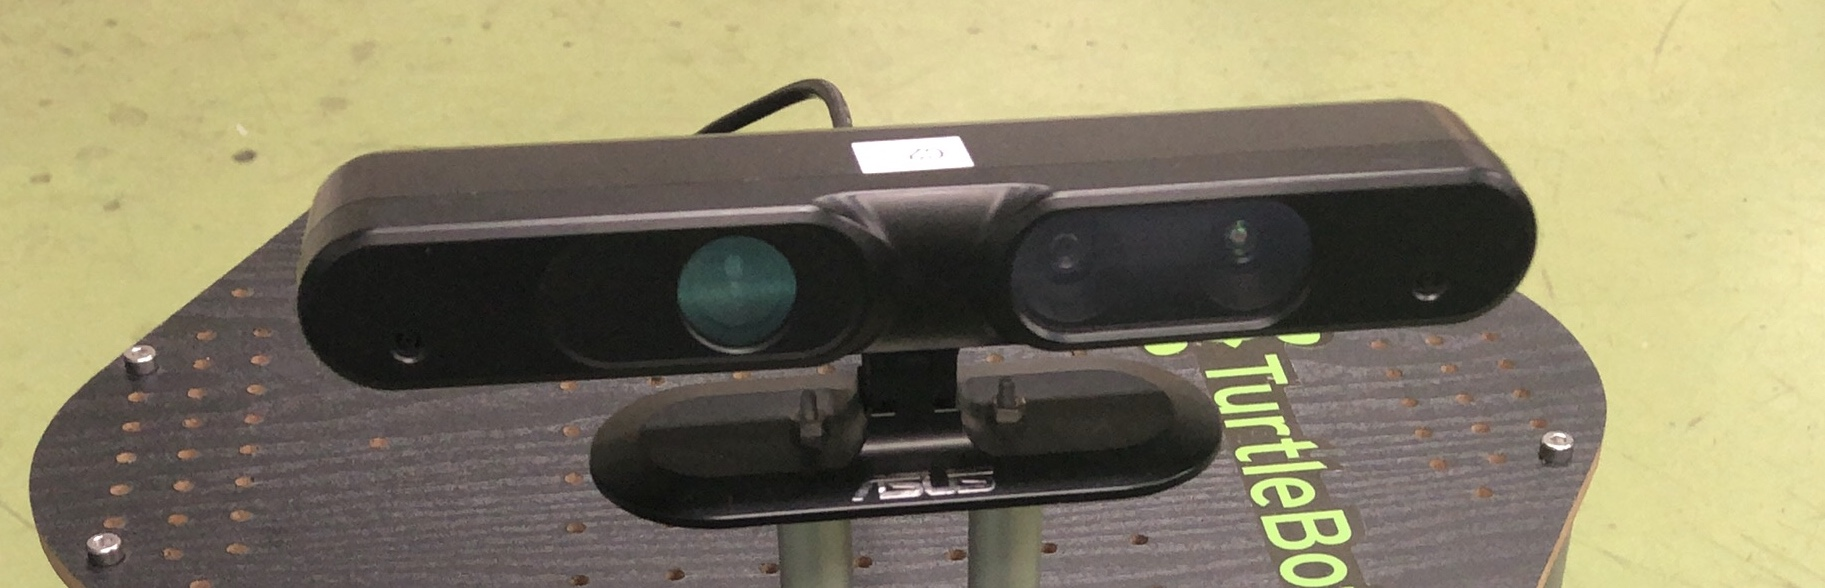
\includegraphics[width = 8cm]{画像/kinect.jpg}
    \caption{カメラセンサー}
    \label{カメラ}
  \end{center}
\end{figure}

\begin{figure}[H]
  \begin{center}
    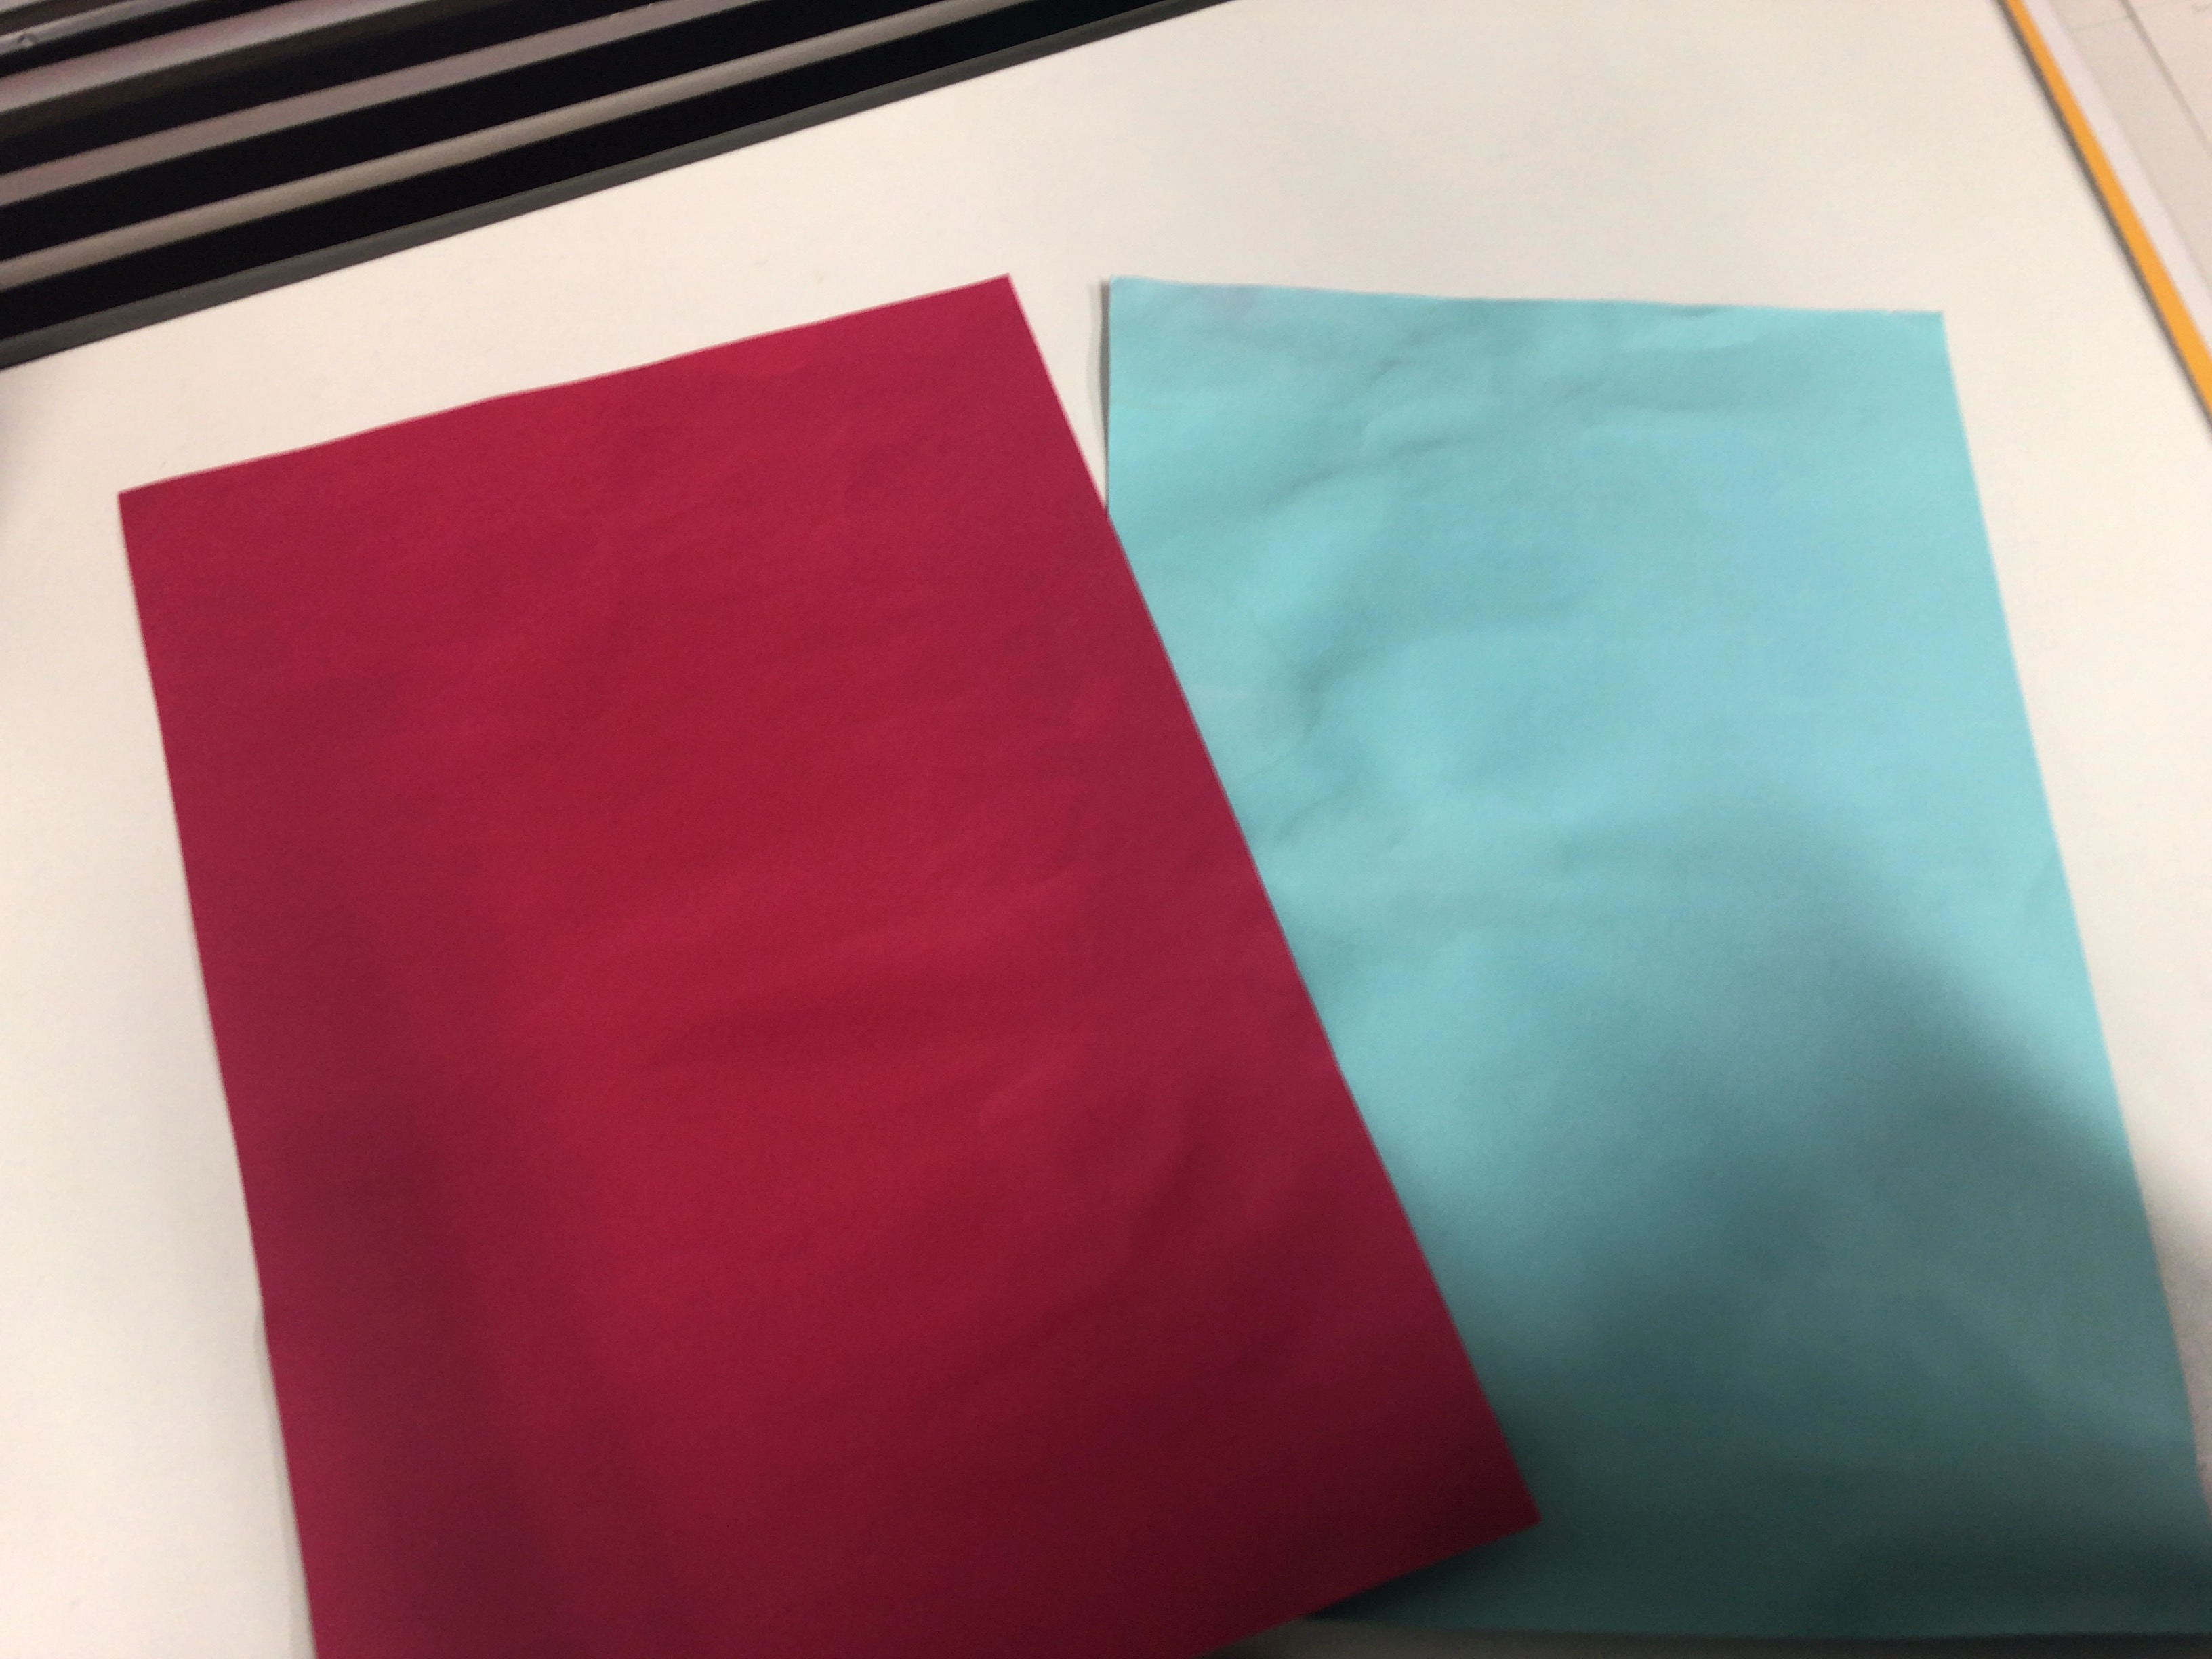
\includegraphics[width = 8cm]{画像/paper.jpg}
    \caption{色の認識に使用した色紙}
    \label{紙}
  \end{center}
\end{figure}

\begin{figure}[H]
  \begin{center}
    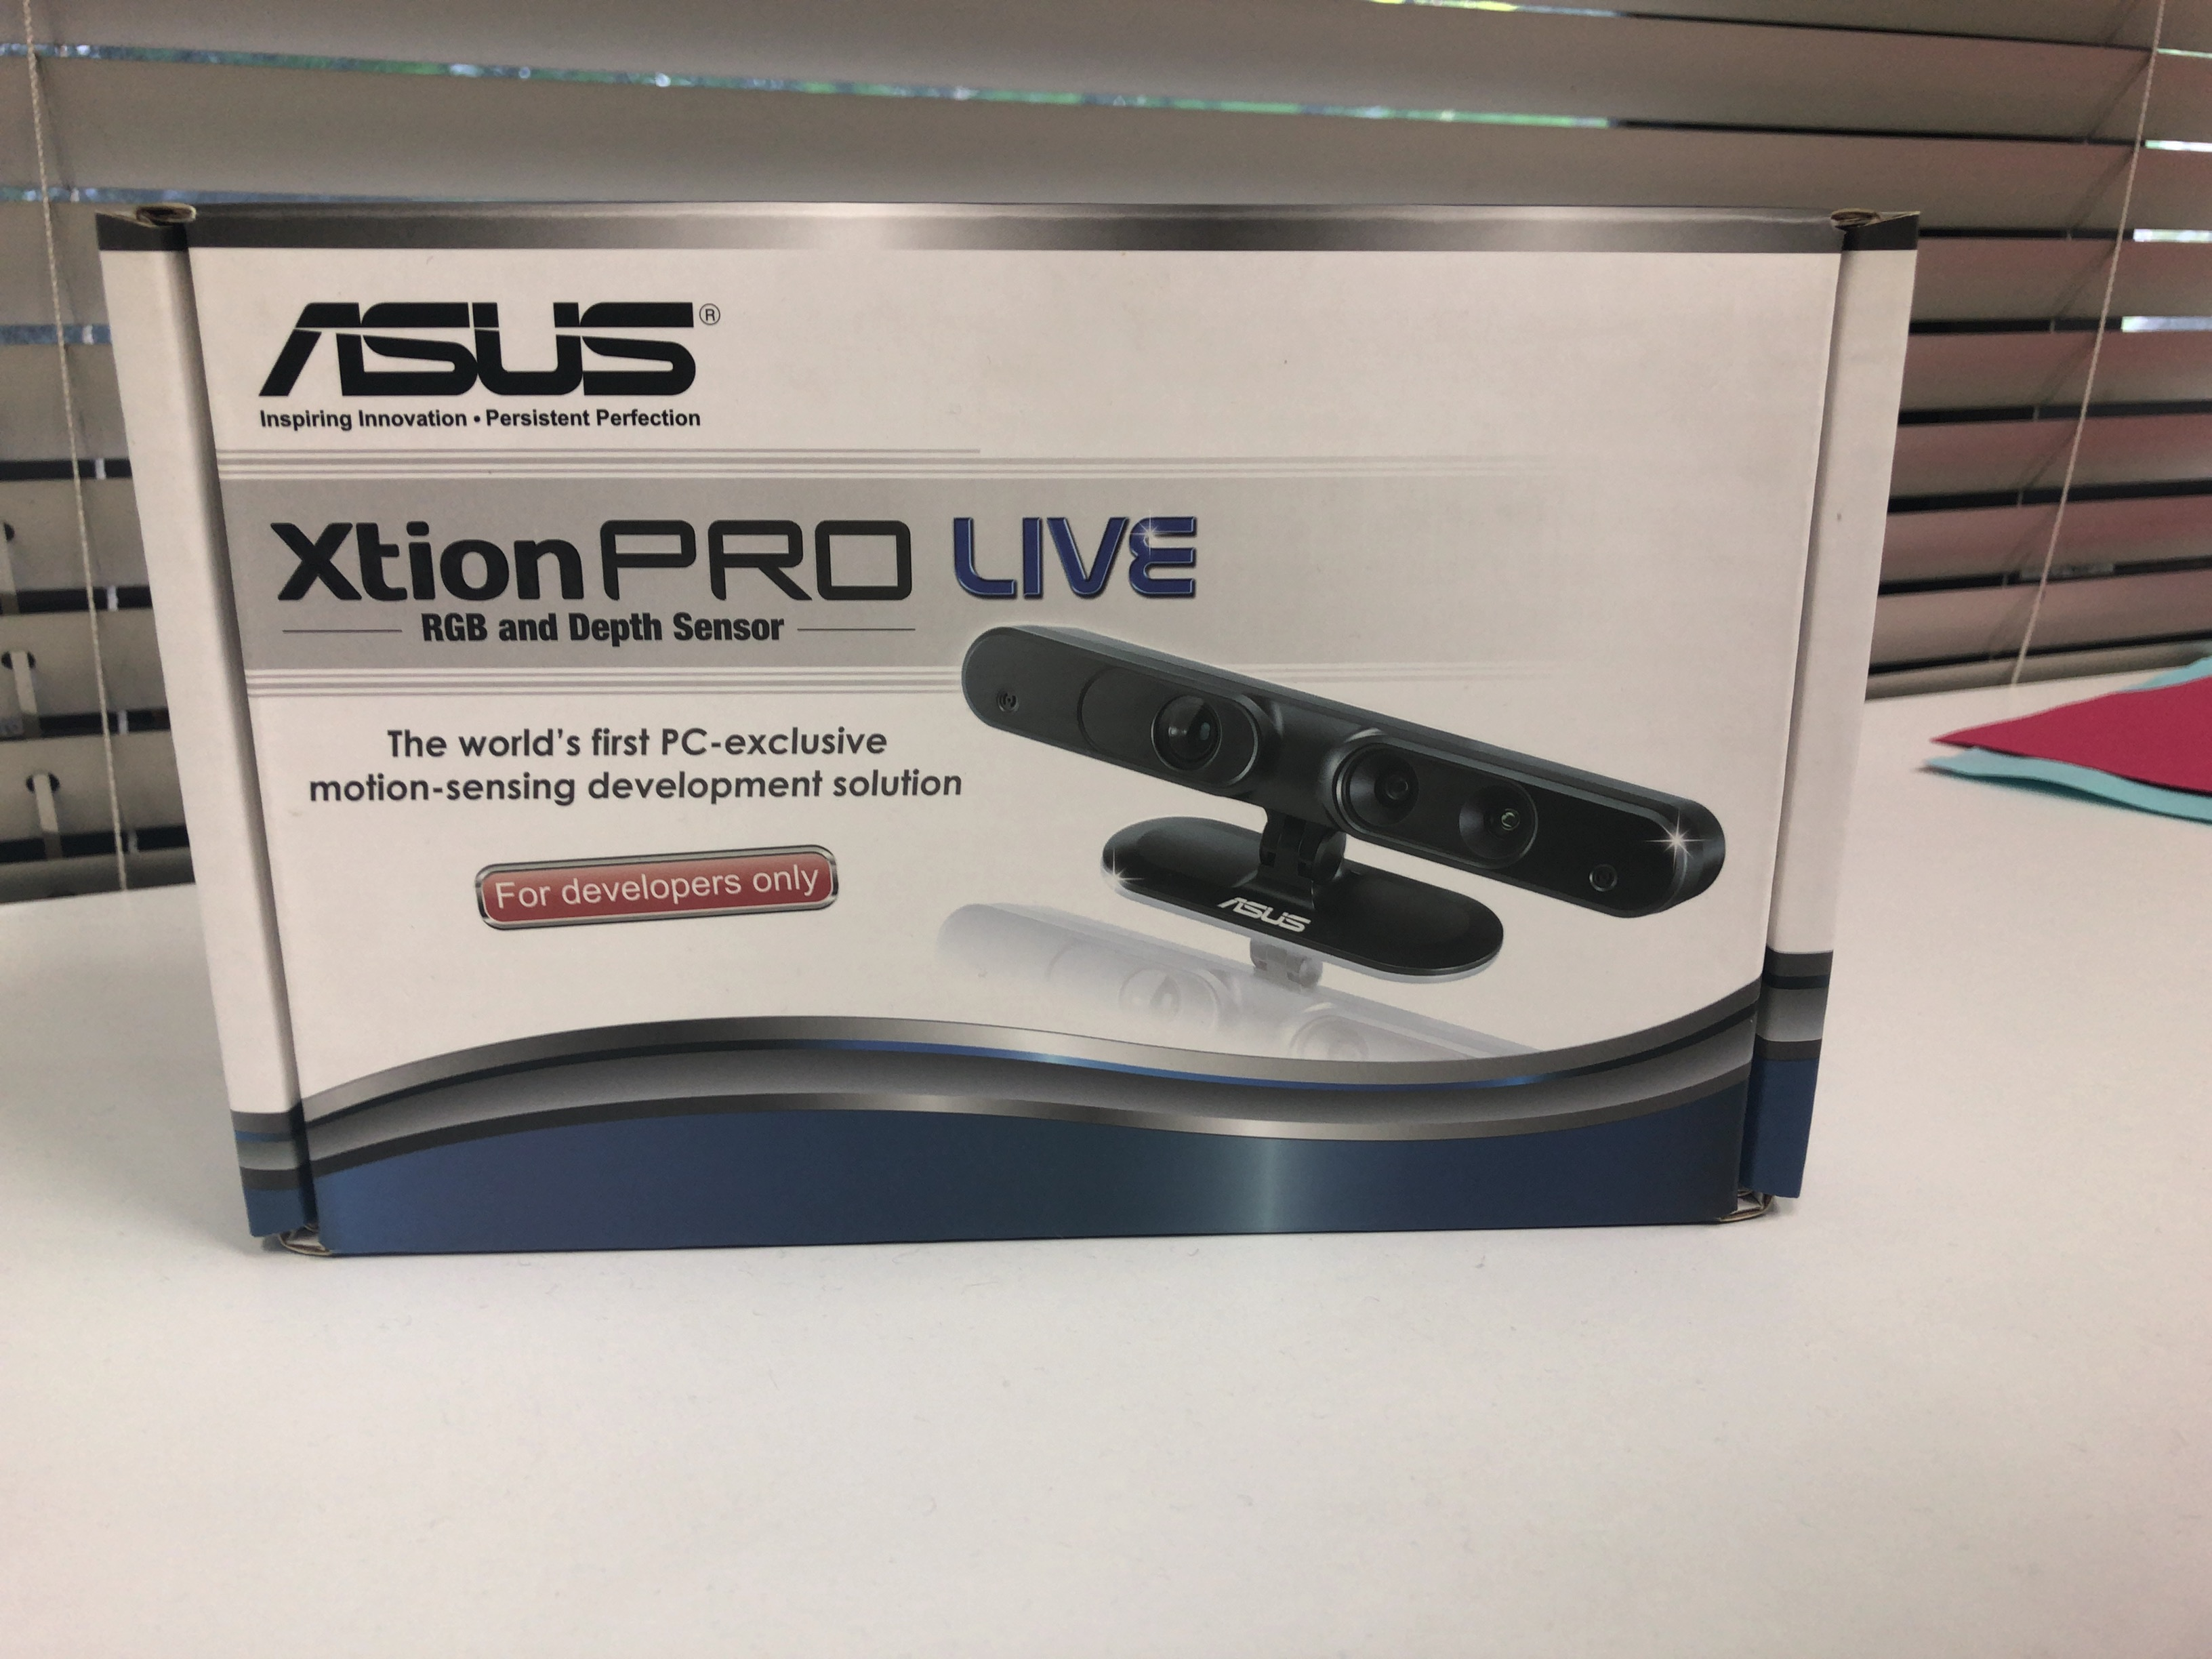
\includegraphics[width = 8cm]{画像/box.jpg}
    \caption{あらかじめ登録した箱}
    \label{箱}
  \end{center}
\end{figure}

\subsection{音声センサー}
あらかじめ音声認識辞書に登録した言葉をコンピュータのマイクに喋りかけると認識する仕組みを用いた.

\subsection{ロボット}
直線移動, 旋回が可能な台車に前述したカメラセンサーを搭載したロボットを用いた(図4). それぞれコンピュータと直接USBケーブルで接続し,
コンピュータと各ノードの通信を行った. 機能として, 移動, 音声認識, 画像認識, 発話が可能である.

\begin{figure}[H]
  \begin{center}
    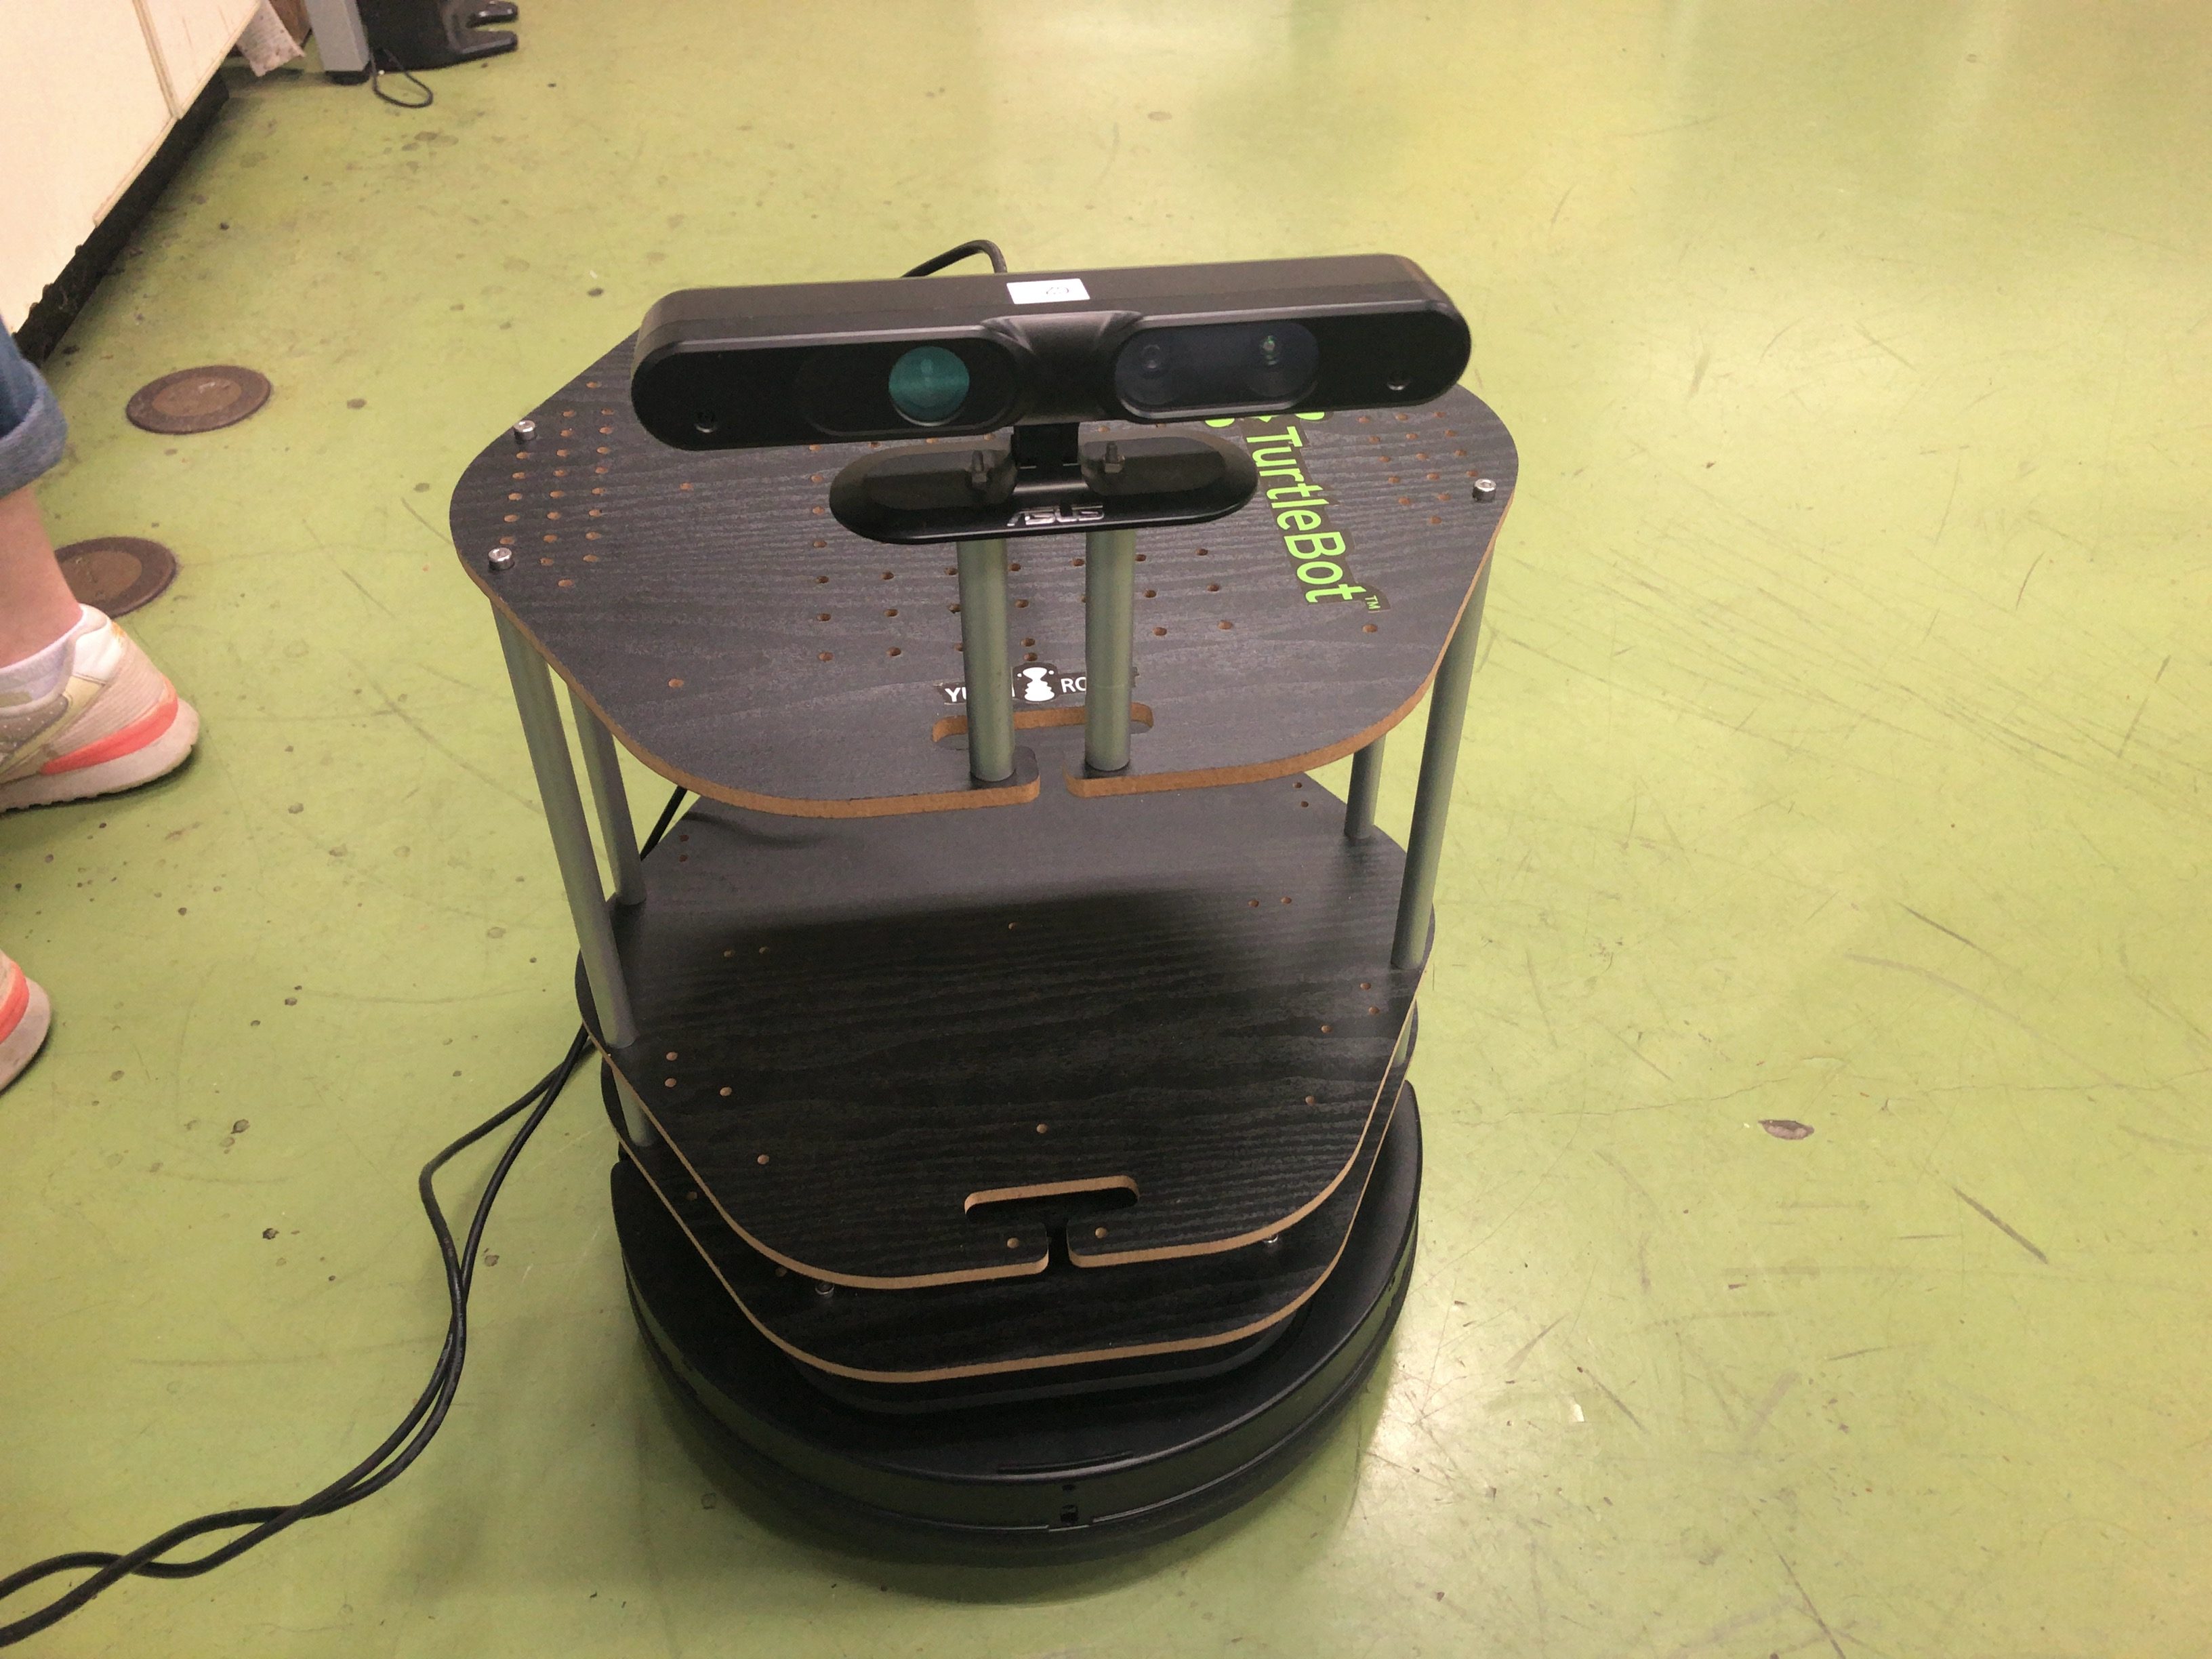
\includegraphics[width = 8cm]{画像/robot.jpg}
    \caption{使用したロボット}
    \label{ロボット}
  \end{center}
\end{figure}

\section{実験課題}
本実験では, 音声で反応する場合と動きで反応する場合の二種類の対話ロボットを課題として扱かった.
\subsection{音声で反応する場合}
音声認識を用いて反応する以下の二つの機能を実装した.
\begin{itemize}
  \item 「さようなら」と喋りかけると, 「ばいばい」という発話とともに首を振る.
  \item 「嫌い」と喋りかけると「もう知りません」と言う発話とともに離れていく.
\end{itemize}

「さようなら」と喋りかけた場合では, 「ばいばい」と発話したのち, 0.5の速度で3秒間右旋回, 0.5の速度で3秒間左旋回
を二回繰り返す命令を書いた.「嫌い」と喋りかけた場合では, 「もう知りません」と発話したのち, 1.0の速度で4.5秒間左旋回
したのちに, 0.1の速度で2秒間直進する命令を書いた.
以下にソースコードを示す.
\begin{lstlisting}[basicstyle=\ttfamily\footnotesize, caption = AudioTest.py, breaklines = true]
# coding: shift-jis
import os
os.system("title AudioTest.py")
from RosClientBin import *
import time

client = RosClient()
client.Connect( "localhost" , "11311" )
client.Subscribe[SpeechInfo]()
client.Publish[SpeechOrder]()

while 1:
    # 音声認識結果の取得
    info = client.GetLastMsg[SpeechInfo]()

    if info:
        print ToString(info.recSpeech), info.isSpeaking
        if ToString(info.recSpeech).find("こんにちは")!=-1:
            # 音声発話命令を送信
            order1 = SpeechOrder()
            order1.utterace = ToBytes("こんにちは")
            order2 = RobotOrder()
            order2.kind = RobotOrder.ORDER_ROTATE;
            order2.data.Add( 1.0 );

            robotstop = RobotOrder()
            robotstop.kind = RobotOrder.ORDER_STOP;

            client.Send( order1 )
            client.Send( order2 )
            time.sleep(9)
            client.Send( robotstop )

        if ToString(info.recSpeech).find("さようなら")!=-1:
            # 音声発話命令を送信
            order1 = SpeechOrder()
            order1.utterace = ToBytes("ばいばい")

            robotright = RobotOrder()
            robotright.kind = RobotOrder.ORDER_ROTATE;
            robotright.data.Add( -0.5 );

            robotleft = RobotOrder()
            robotleft.kind = RobotOrder.ORDER_ROTATE;
            robotleft.data.Add( 0.5 );

            robotstop = RobotOrder()
            robotstop.kind = RobotOrder.ORDER_STOP;

            client.Send( order1 )
            for i in range(2):
                client.Send( robotright )
                time.sleep(3)
                client.Send( robotleft )
                time.sleep(3)
            client.Send( robotstop )

        if ToString(info.recSpeech).find("嫌い")!=-1:
            # 音声発話命令を送信
            order1 = SpeechOrder()
            order1.utterace = ToBytes("もう知りません")
            order2 = RobotOrder()
            order2.kind = RobotOrder.ORDER_ROTATE;
            order2.data.Add( 1.0 );

            robotstop = RobotOrder()
            robotstop.kind = RobotOrder.ORDER_STOP;

            robotforward = RobotOrder()
            robotforward.kind = RobotOrder.ORDER_MOVE_FORWARD;
            robotforward.data.Add( 0.1 );

            client.Send( order1 )
            client.Send( order2 )
            time.sleep(4.5)
            client.Send( robotforward )
            time.sleep(2)
            client.Send( robotstop )

        if ToString(info.recSpeech).find("前へすすめ")!=-1:
            # 音声発話命令を送信
            order1 = RobotOrder()
            order2 = SpeechOrder()
            order1.kind = RobotOrder.ORDER_MOVE_FORWARD;
            order1.data.Add( 0.1 );
            order2.utterace = ToBytes("了解")
            client.Send( order2 )
            client.Send( order1 )

        if ToString(info.recSpeech).find("止まれ")!=-1:
            # 音声発話命令を送信
            order1 = RobotOrder()
            order2 = SpeechOrder()
            order1.kind = RobotOrder.ORDER_STOP;
            order2.utterace = ToBytes("了解")
            client.Send( order2 )
            client.Send( order1 )
\end{lstlisting}

\subsection{動きで反応する場合}
人間骨格の認識を用いて, 以下の機能を実装した.
\begin{enumerate}
  \item 右手が上がると「I have a pen」と発話する.
  \item 左手が上がると「I have an apple」と発話する.
  \item 右手が前にあると「apple pen」と発話する.
\end{enumerate}
以下にソースコードを示す.
\begin{lstlisting}[basicstyle=\ttfamily\footnotesize, caption = VisionTest.py, breaklines = true]
# coding: shift-jis
import os
os.system("title VisionTest.py")
from RosClientBin import *
import time

client = RosClient()
client.Connect( "localhost" , "11311" )
client.Subscribe[Skeltons]()
client.Subscribe[Objects]()
client.Subscribe[Faces]()
client.Subscribe[ColorBlobs]()

while 1:
    # 骨格情報を取得
    skeltons = client.GetLastMsg[Skeltons]()
    if skeltons:
        if skeltons.data.Count:
            rightUp = False
            leftUp = False
            rightFront = False
            leftFront = False
            rightSide = False
            leftSide = False

            # 手の座標と頭の座標を基準に手の状態を識別
            if skeltons.data[0].joints[Skelton.SKEL_RIGHT_HAND].y - skeltons.data[0].joints[Skelton.SKEL_HEAD].y > 0: rightUp = True;
            if skeltons.data[0].joints[Skelton.SKEL_LEFT_HAND].y - skeltons.data[0].joints[Skelton.SKEL_HEAD].y > 0: leftUp = True;

            if skeltons.data[0].joints[Skelton.SKEL_HEAD].z - skeltons.data[0].joints[Skelton.SKEL_RIGHT_HAND].z > 300: rightFront = True;
            if skeltons.data[0].joints[Skelton.SKEL_HEAD].z - skeltons.data[0].joints[Skelton.SKEL_LEFT_HAND].z > 300: leftFront = True;

            if skeltons.data[0].joints[Skelton.SKEL_RIGHT_HAND].x - skeltons.data[0].joints[Skelton.SKEL_RIGHT_SHOULDER].x < -300: rightSide = True;
            if skeltons.data[0].joints[Skelton.SKEL_LEFT_HAND].x - skeltons.data[0].joints[Skelton.SKEL_LEFT_SHOULDER].x > 300: leftSide = True;

            print "右手:",
            if rightUp:
                print "上",
                order = SpeechOrder()
                order.utterace = ToBytes("あいはぶあぺん")
                client.Send( order )
                time.sleep(4)

            if rightFront:
                print "前",
                order = SpeechOrder()
                order.utterace = ToBytes("んーあっぽーぺーん")
                client.Send( order )
                time.sleep(4)
            if rightSide:     print "横",
            print

            print "左手:",
            if leftUp:
                print "上",
                order = SpeechOrder()
                order.utterace = ToBytes("あいはぶああっぽー")
                client.Send( order )
                time.sleep(4)
            if leftFront:   print "前",
            if leftSide:    print "横",
            print

    # 物体検出結果受信
    objects = client.GetLastMsg[Objects]()
    if objects:
        for i in range( objects.data.Count ):
            print "物体検出 id:", objects.data[i].id, " pos:",objects.data[i].pos.x, objects.data[i].pos.y,objects.data[i].pos.z

    # 顔検出結果受信
    faces = client.GetLastMsg[Faces]()
    if faces:
        for i in range( faces.data.Count ):
            print "顔検出 id:", faces.data[i].id, " pos:",faces.data[i].pos.x, faces.data[i].pos.y,faces.data[i].pos.z

    # 色検出結果を受信
    color = client.GetLastMsg[ColorBlobs]()
    if color:
        for i in range( color.data.Count ):
            print "色検出 id:" , color.data[i].id, " pos:",color.data[i].pos.x, color.data[i].pos.y, color.data[i].pos.z
\end{lstlisting}

\section{考察}
\subsection{音声で反応する場合}
左右と旋回するフローを二回繰り返す動きと$180^{\circ}$旋回した後に直進する動きを実装した.
どちらも速度指定による旋回を用いたので, 旋回角度を正確に指定することができなかった.
速度指定による旋回では, 指定した速度に到達するまでの加速に時間がかかるため, 同じ速度命令を出したとしても
命令開始時のロボットの旋回速度によって挙動が変化してしまった. 時間上の都合で, 角度指定による旋回が正常に動作させられなかったが, 角度指定による旋回を用いた方が良いと考える.

\subsection{動きで反応する場合}
 左右の手の位置に応じた発話を実装した. 今回, ロボットは発話するのみだったが, 人間の動きに合わせて
 発話と動作をするという実装をさせてみたい. また, それぞれのif文の中にtime.sleep()命令を書くことで重複して発話することを
 抑止させたが, 休止時間が経過するまで次の動作に対する発話が実行できないので, 重複発話を防ぎつつ, 動作があった場合には
 すぐに反応できる実装を実現できればより良いと考える.

\subsection{まとめ}
音声で反応する場合と動きで反応する場合の二種類の動作の実装を行った. 具体的な実装を考える上で, ロボットがどのような動き,
反応をすると面白いか, 面白いロボットとはなんたるかを第一として実装方針を立てた. ロボットは基本的に人間が命令を送らなければ何もできないのが当たり前であり,
命令されたことを行うのも当たり前である. そこで, 命令されていてもまるで命令されていないような動きこそが面白い対話なのではないかと考えた.
音声で反応する場合では, 人間が話したことに対して感情を表現. 動きで反応する場合では, 人間の動きに反応し, 協力して一つの作品を作る協力という対話を表現した.
実際に実装してみたところ, ロボットの動きに対して笑みがこぼれ, ロボットとの心理的な距離の縮まりや親しみを感じることができたため, 実装方針と目的は概ね達成されたと考える.

\section{参考文献}
\noindent [1]知能機械工学基礎実験,電気通信大学  知能機械工学科 \\ \relax
[2]BRILLIANTSERVICE TECHBLOG http://bril-tech.blogspot.com/2016/10/ros1-robot-operating-system.html\\ \relax
[3]NTTテクノクロスHP http://www.v-series.jp/speechrec/about\_asr.html \\ \relax
\end{document}
